\documentclass[11pt]{article}
\usepackage{enumerate}
\usepackage{fullpage}
\usepackage{fancyhdr}
\usepackage{tikz}
\usepackage{amsmath, amsfonts, amsthm, amssymb}
\setlength{\parindent}{0pt}
\setlength{\parskip}{5pt plus 1pt}
\pagestyle{empty}

\def\indented#1{\list{}{}\item[]}
\let\indented=\endlist

\newcounter{questionCounter}
\newcounter{partCounter}[questionCounter]
\newenvironment{question}[2][\arabic{questionCounter}]{%
    \setcounter{partCounter}{0}%
    \vspace{.25in} \hrule \vspace{0.5em}%
        \noindent{\bf #2}%
    \vspace{0.8em} \hrule \vspace{.10in}%
    \addtocounter{questionCounter}{1}%
}{}
\renewenvironment{part}[1][\alph{partCounter}]{%
    \addtocounter{partCounter}{1}%
    \vspace{.10in}%
    \begin{indented}%
       {\bf (#1)} %
}{\end{indented}}

%%%%%%%%%%%%%%%%%%%%%%%%%%%%%%%%%%%%%%%%%%%%%%%%%%%%%%%%%%%
\newcommand{\myname}{Shashank Singh}
\newcommand{\myandrew}{sss1@andrew.cmu.edu}
\newcommand{\myclass}{21-484A Graph Theory}
\newcommand{\myhwnum}{2}
\newcommand{\duedate}{Friday, February 24, 2012}
%%%%%%%%%%%%%%%%%%%%%%%%%%%%%%%%%%%%%%%%%%%%%%%%%%%%%%%%%%%

\begin{document}
\thispagestyle{plain}

{\Large Homework \myhwnum} \\
\myclass \\
Name: \myname \\
Email: \myandrew \\
Due: \duedate

\begin{question}{Problem 1}
Let $a$ be the number of vertices in $T$ of degree $1$, let $b$ be the number
of vertices in $T$ of degree $3$, and let $e = |E(T)|$. Since $T$ is a tree,
$e = n - 1$. Furthermore, \[2e = \sum_{v \in V(T)} \mbox{deg}(v) = a + 3b.\]
Finally, $a + b = n$. Solving this system of three linear equations in three
variables gives $a = \frac{n + 2}{2}$, $b = \frac{n - 2}{2}$. Thus, the number
of leaves in $T$ is \[a = \mbox{\fbox{$\displaystyle \frac{n + 2}{2}$.}}\]
\end{question}

\begin{question}{Problem 2}
Suppose $G$ is a graph with at least $4$ vertices, such that the subgraph
induced by any $3$ vertices in $G$ is a tree. Suppose, for sake of
contradiction, that $G$ contains at least $|V(G)| \geq 5$. Then, let
$v_1,v_2,\ldots,v_5$ be distinct vertices in $G$, and let $H$ be the subgraph
of $G$ induced by $v_1,v_2,\ldots,v_5$. Then, $H$ also has the property that,
the subgraph of $H$ induced by any $3$ vertices in $H$ is a tree. For any
distinct $t,u,v \in \{v_1,v_2,\ldots,v_5\}$, let $T_{t,u,v}$ be the subgraph
of $H$ induced by $t,u,v$. Since $T_{v_1,v_2,v_3}$ is a tree, it contains
$3 - 1 = 2$ edges; without loss of generality, $v_1v_2$ and $v_2v_3$ are in
$H$. If $v_2v_5$ were in $H$, then neither $v_1v_5$ nor $v_3v_5$ could be in
$H$ (since, if either were the case, then either $T_{v_1,v_2,v_5}$ or
$T_{v_3,v_2,v_5}$ would have $3$ edges and thus not be a tree); therefore,
$v_2v_5$ is not an edge in $H$. A similar argument shows that $v_2v_4$ is not
an edge in $H$. Then, however, $T_{v_2,v_4,v_5}$ contains at most $1$ edge,
contradicting the hypothesis that $T_{v_2,v_4,v_5}$ is a tree. Thus, $G$
contains at most $4$ vertices, and so it contains exactly $4$ vertices. Thus,
by inspection of the $11$ distinct unlabeled graphs on $4$ vertices, it can
be seen that $G$ must be of the form of the following graph:

\begin{center}
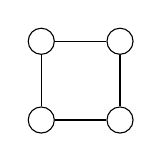
\begin{tikzpicture}
  [scale=1,auto=center,every node/.style={draw,circle}]
  \node (n2) at (1,1)  {};
  \node (n1) at (2,1)  {};
  \node (n3) at (1,2)  {};
  \node (n4) at (2,2)  {};
  \foreach \from/\to in {n1/n2,n2/n3,n3/n4,n4/n1}
    \draw (\from) -- (\to);
\end{tikzpicture}
\end{center}
$\blacksquare$
\end{question}

\begin{question}{Problem 3}
Let $G$ be a connected graph, and suppose some $e \in E(G)$ is a bridge. Let
$v_1,v_2$ be the endpoints of $e$. Then, by definition of bridge, all walks
from $v_1$ to $v_2$ contain $e$ (since, if $e$ is removed from $G$, there are
no walks from $v_1$ to $v_2$). Suppose $T$ is a spanning tree of $G$. Then,
$T$ must contain a walk from $v_1$ to $v_2$. Therefore, $T$ must contain $e$.

Suppose, on the other hand, that, for some edge $e$ in $G$, every spanning
tree $T$ of $G$ contains $e$. Suppose, for sake of contradiction, that $e$ is
not a bridge. Then, by definition of bridge, letting $H$ be the graph
resulting from removing $e$ from $G$, $H$ is connected. Thus, $H$ has a
spanning tree $T$. Since $V(H) = V(G)$, $T$ is also a spanning tree of $G$.
However, since $T$ is a spanning tree of $H$, $e$ is not in $T$, contradicting
the given that $e$ is in every spanning tree of $G$.

Therefore, an edge $e$ in a connected graph $G$ is a bridge if and only if $e$
is in every spanning tree of $G$. \qquad $\blacksquare$
\end{question}

\begin{question}{Problem 4}
Let $G$ be a connected graph, let $n = |V(G)|$, and let $T$ and $T^{\prime}$
be two spanning trees of $G$. Let $k$ be the number of edges that are in
$T^{\prime}$ but not in $T$ (i.e., $k = |E(T^{\prime}) \backslash E(T)|$).
We proceed by induction on $k$.

If $k = 0$, then, since $|E(T^{\prime})| = n - 1 = |E(T)|$,
$E(T^{\prime}) = E(T)$, so that $T = T^{\prime}$, and the sequence $T$
fulfills the desired properties.

Suppose that, for some $k \in \mathbb{N}$, $\forall$ spanning trees $T^{\prime}$ of
$G$ such that $|E(T^{\prime}) \backslash E(T)| \leq k$, there exists a
sequence $T = T_1,T_2,\ldots,T_k = T^{\prime}$ such that
\[|E(T_i) \cap E(T_{i + 1})| \geq n - 2,
                              \forall i \in \mathbb{N}, 0 \leq i \leq k - 1.\]
Suppose that, for some $T^{\prime}$,
$|E(T^{\prime}) \backslash E(T)| \leq k + 1$.
Then, $\exists e_1 \in E(T^{\prime})$ such that $e_1 \not \in E(T)$. Let $H$
be the graph resulting from adding $e_1$ to $T$. Since $T$ is a tree, $H$
contains a cycle. Thus, since $T^{\prime}$ is a tree, there is some edge $e_2$
in this cycle such that $e_2 \not \in T^{\prime}$. Let $T_1$ be the graph
resulting from removing $e_2$ from $H$. Then, since $T_1$ is a connected graph
on $n$ vertices with $n - 1$ edges, $T_2$ is a tree. Furthermore,
$|E(T_1)\cap E(T)|\geq n - 2$, and $|E(T^{\prime})\backslash E(T_1)|\leq k$.
Then, by the inductive hypothesis, there exists a sequence
$T_1, T_2, \ldots, T_m = T^{\prime}$ such that,
$|E(T_i) \cap E(T_{i + 1})| \geq n - 2$, $\forall i \in \mathbb{N}$ with
$1 \leq i \leq m - 1$, so that the sequence
$T = T_0,T_1,T_2,\ldots,T_m = T^{\prime}$ has the desired properties.
Thus, by the Principle of Mathematical Induction, the claim in question holds
$\forall k \in \mathbb{N}$. \qquad $\blacksquare$
\end{question}

\begin{question}{Problem 5}
The number labeled trees on $n$ vertices is the same as the number of spanning
trees of $K_n$, the complete graph on $n$ vertices, since any spanning tree of
$K_n$ is by definition a tree on $n$ vertices, and every tree on $n$ vertices
is a subgraph of $K_n$. By definition,
\[L_{K_n} =
\left[\begin{array}{ccccc}
 n - 1  &   -1   &   -1   & \cdots &   -1   \\
   -1   & n - 1  &   -1   & \cdots &   -1   \\
   -1   &   -1   & n - 1  & \cdots &   -1   \\
 \vdots & \vdots & \vdots & \ddots & \vdots \\
   -1   &   -1   &   -1   & \cdots & n - 1  \\
\end{array}\right],\]
where $L_{K_n}$ is of size $n \times n$. The $(n - 1)$ vectors

\[
\left[\begin{array}{c}
  1     \\
  -1    \\
  0     \\
  0     \\
 \vdots \\
  0
\end{array}\right],
\left[\begin{array}{c}
  0     \\
  1     \\
  -1    \\
  0     \\
 \vdots \\
  0
\end{array}\right], \cdots,
\left[\begin{array}{c}
  0     \\
  0     \\
  0     \\
 \vdots \\
  1     \\
  -1
\end{array}\right], \in \mathbb{R}^n\]

are eigenvectors of $L_{K_n}$, each of eigenvalue $n$. Thus, by Kirchoff's
Theorem, the number of spanning trees of $K_n$ is
$\frac{1}{n}n^{n - 1} = n^{n - 2}$, proving Cayley's formula.
\qquad $\blacksquare$
\end{question}

\begin{question}{Problem 6}
Let $G$ be a graph, $n = |V(G)|$, $e = |E(G)|$. Order the vertices of $G$ as
$v_1,v_2,\ldots,v_n$, and the edges of $G$ $e_1,e_2,\ldots,e_m$, so that,
letting $M = E_G$, for $i \in [n]$, $j \in [m]$, $M_{v_i,e_j}$,
$M_{i,j} = -1$ if the source of $e_j$ is $v_i$, $M_{i,j} = 1$ if the
destination of $e_i$ is $v_i$, and $M_{i,j} = 0$ otherwise. Let $L = L_G$.
Then, $\forall i \in [n]$, $\left(MM^T\right)_{i,i}$ is the sum of the squares
of the elements of the $i^{th}$ row of $M$; since there is a $1$ or a $(-1)$
in this row for each incoming or outgoing edge of $v_i$,
$\left(MM^T\right)_{i,i} =$ deg$(v_i)$, so that
$\left(MM^T\right)_{i,i} = L_{i,i}$.

$\forall i,j \in [n]$ with $i \neq j$, $\left(MM^T\right)_{i,j}$ is $-1$ if,
for some $k \in [m]$, the $k^{th}$ entry in both the $i^{th}$ and $j^{th}$
rows of $M$ are non-zero (i.e., one is $1$ and the other is $(-1)$). By
definition of $M$, this occurs precisely when the $e_k$ has $v_i$ and $v_j$ as
endpoints, so that this happens precisely when there is an edge between $v_i$
and $v_j$. Therefore, by definition of the $L$,
$\left(MM^T\right)_{i,j} = L_{i,j}$.

Thus, $\forall i,j \in [n]$, $\left(MM^T\right)_{i,j} = L_{i,j}$, so that
$MM^T = L$. \qquad $\blacksquare$
\end{question}

\begin{question}{Problem 7}
For $k = 0$, $A^k = I_n$ (the $n \times n$ identity matrix. Since, for
$(i,j) \in [n] \times [n]$, $I_{i,j} = 1$ if and only if $i = j$, and there
exists a (necessarily unique) walk of length $0$ from vertex $i$ to vertex $j$
in $G$, if and only if $i = j$, the claim in question holds for $k = 0$.

Suppose that, for some $k \in \mathbb{N}$, $\forall (i,j) \in [n] \times [n]$,
$A^k_{i,j}$ gives the number of walks of length $k$ from vertex $i$ to vertex
$j$ in $G$. $\forall (v,u) \in [n] \times [n]$, let $e_{v,j} = 1$ if and only
if $v$ and $j$ are adjacent in $G$ ($e_{v,j} = 0$ otherwise).
$\forall v \in [n]$ the number of walks of length $(k + 1)$ from $i$ to $j$
whose last edge is $vj$ is the same as the number of walks of length $k$ from
$i$ to $v$ if $v$ is adjacent to $j$ in $G$, and $0$ otherwise. Thus,
partitioning the walks of length $(k + 1)$ from $i$ to $j$ in $G$ by their
last edge shows that the number of such walks is given by
\[\sum_{v \in V(G)} A^k_{v,j}e_{v,j} = \sum_{v = 1}^n A^k_{v,j}e_{v,j}.\]
$\forall (i,j) \in [n] \times [n]$, by construction of $e_{i,j}$ and the
definition of the adjacency matrix, $A_{i,j} = e_{i,j}$. Thus, matrix
multiplication gives
\[A^{k + 1}_{i,j}
 = \left(A^kA\right)_{i,j}
 = \sum_{i = 1}A^k_{i,j}A_{i,j}
 = \sum_{i = 1}A^k_{i,j}e_{i,j},\]
so that $A^{k + 1}_{i,j}$ is the number of walks of length $(k + 1)$ from $i$
to $j$ in $G$. Thus, by the Principle of Mathematical Induction,
$\forall k \in \mathbb{N}$, $\forall (i,j) \in [n] \times [n]$, $A^k_{i,j}$
gives the number of walks of length $k$ from $i$ to $j$ in $G$.
\qquad $\blacksquare$
\end{question}

\begin{question}{Problem 8}
By Kirchoff's Theorem, the following matlab code gives the desired quantity as
output (\texttt{m} is defined as $L_G$):

\begin{verbatim}
>> m = [[6,0,-1,-1,-1,-1,-1,-1];
        [0,6,-1,-1,-1,-1,-1,-1];
        [-1,-1,6,0,-1,-1,-1,-1];
        [-1,-1,0,6,-1,-1,-1,-1];
        [-1,-1,-1,-1,6,0,-1,-1];
        [-1,-1,-1,-1,0,6,-1,-1];
        [-1,-1,-1,-1,-1,-1,6,0];
        [-1,-1,-1,-1,-1,-1,0,6]];
>> eigenvalues = eig(m);
>> n = 8;
>> prod(eigenvalues(2:8))/n             %the first eigenvalue is 0

ans =

      82944
\end{verbatim}
Thus, the number of spanning trees of $G$ is \fbox{$82944$.}
\end{question}
\end{document}
